\documentclass[a4paper,fleqn]{cas-sc}
%%%%%%%%%%%%%%% Declare Package: %%%%%%%%%%%%%
% \usepackage[authoryear,longnamesfirst]{natbib}
\usepackage{ragged2e}% Align macro package
\usepackage{amsmath}%math equation IMPORTANT!!!
\usepackage{amssymb}
\usepackage{nomencl}% use nomenclature package
\usepackage{graphicx}% to insert graph
\graphicspath{{Figures/}}% the path of graphs1
% \usepackage{bm}% bold font special for math formulas
\usepackage{caption}
\usepackage[raggedright,nooneline,FIGTOPCAP]{subfigure}% need to call both packages: subcaption and caption at the same time
\captionsetup{figurename=Fig.,
labelsep=period,
font={bf,footnotesize},
center}% \usepackage{ifthen}% use condition judgement
\usepackage{setspace}
\DeclareMathOperator\dif{d\!}% the derivative operator d
\usepackage{xfrac}% small fraction, for example 1/2
\usepackage{multirow,booktabs} %three-line table
\usepackage{array} % fixed width and auto newline(wrap) as well centering
\usepackage{float}
\usepackage{callouts}
\usepackage{microtype}% improve the intervals between words to make typing more beautiful
\usepackage{lineno,hyperref}% display line number, use hyper reference

%%%%%%%%%%%%%% Title and author: %%%%%%%%%%%%%
\begin{document}
\let\WriteBookmarks\relax
\def\floatpagepagefraction{1}
\def\textpagefraction{.001}
\shorttitle{Unequal planet load sharing}
\shortauthors{Feng et al.}

\title[mode = title]{A vibration signal model of planetary gearboxes with unequal load sharing among planets}
\author[1]{Haoqun Ma}[type=editor]
\address[1]{University of Science and Technology Beijing, No.30, Xueyuan Road, Haidian District, Beijing.}
\author[1]{Zhipeng Feng}[type=co-ordinator,orcid=0000-0002-3403-4386]
\cormark[1]
\ead{fengzp@ustb.edu.cn}
\cortext[cor1]{Corresponding author}
%%%%%%%%%%%%%% Abstract %%%%%%%%%%%%%%%%%%%%%%
\begin{abstract}
    This template helps you to create a properly formatted \LaTeX\ manuscript.
\end{abstract}
%%%%%%%%%%%%%%%%% Highlights %%%%%%%%%%%%%%%%%%%%%%
\begin{highlights}
    \item Research highlights item 1
    \item Research highlights item 2
    \item Research highlights item 3
\end{highlights}
%%%%%%%%%%%%%%%% keywords %%%%%%%%%%%%%%%%%%
\begin{keywords}
    Unequal load sharing \sep\ planetary gearbox \sep\ Signal model
\end{keywords}
    
%%%%%%%%%%%%%% Begin document: %%%%%%%%%%%%%%%
\maketitle
%%%%%%%%%%%%%%% Custom commands: %%%%%%%%%%%%
%%%%%%%%%%%%%%% Introduction %%%%%%%%%%%%%%%%
\section{Introduction}
\par Planets split power transmitted from the input sun gear into paralleled paths so that planetary gearboxes can withstand heavy load in a compact volume. While the special structure bring about unequal load sharing among planets.
%%%%%%%%%%%%%%% References %%%%%%%%%%%%%%%%%
%%%%%%%%%%%%%%% Principle %%%%%%%%%%%%%%%%
\section{Signal model}
\begin{enumerate}[1.]
    \item Planetary gearboxes have different configuration with similar layouts.
    \item In this paper, we only consider the case where ring gear is fixed. (refer to the paper mentioning the sun or carrier as the fixed central part)
    \item The vibration sensor is mounted on the stationary ring gear.
    \item The vibration mainly origins the the time-varying stiffness gear meshing. When the planet gears engage with the ring gear or sun gear, the number of the involved tooth varies with the relative rotation between gears. Thus, their contact stiffness changes at the same time. If the transmission load proximately remain constant, this system is pure parametric excited. (Add a reference about instability) 
    \item Specially, the torque load transferred from the central components in planetary gearboxes is split into parallel paths formed by the planets. Because of the inevitable manufacturing and assembling errors of pinholes or bearings, there are usually differences in the position of pinholes and the shape of planets. The load sharing among planets is non-uniform (collect other reasons from the Sigh's paper).
    \item Another common phenomenon in planetary gearboxes is the difference in meshing phases between ring-planet and sun-planet. When this situation coincides with the load sharing inequality, a complex couple mechanism of time-varying load sharing emerges, rising extra vibrations.
    \item For an individual planet, the vibration signal model can be written as
    \begin{equation}
        J \cdot \ddot{\theta}(t) + k(t) \cdot \left[\theta(t)-L(t) \right] = 0,
    \end{equation}
    where \(J\) is rotational inertia of the machine, \(\theta(t)\) is the shaft angular, \(\ddot{\theta}(t)\) is the rotational acceleration, \(k(t)\) is time-varying meshing stiffness, \(L(t)\) is the external load.
    \item Taking all planets into account, the above vibration model can be revised as
    \begin{equation}
        J \cdot \ddot{\theta}(t) + \sum^{M}_{i=1} \left\{ k_i(t) \cdot \left[\theta(t)-L(t)+\epsilon_i \right] \right\} = 0,
    \end{equation}
    where \(M\) is the number of planets, \(k_i(t)\) is the meshing stiffness of \(i\)-th planet, \(\epsilon_i\) is the angular shift away from its normal position of \(i\)-th planet (here we assume \(\epsilon_2\neq 0\)). A translational spring-mass system illustrate the above vibration model in Fig. \ref{fig:vibration_system_of_spring_mass}.
    \begin{figure*}
        \centering
        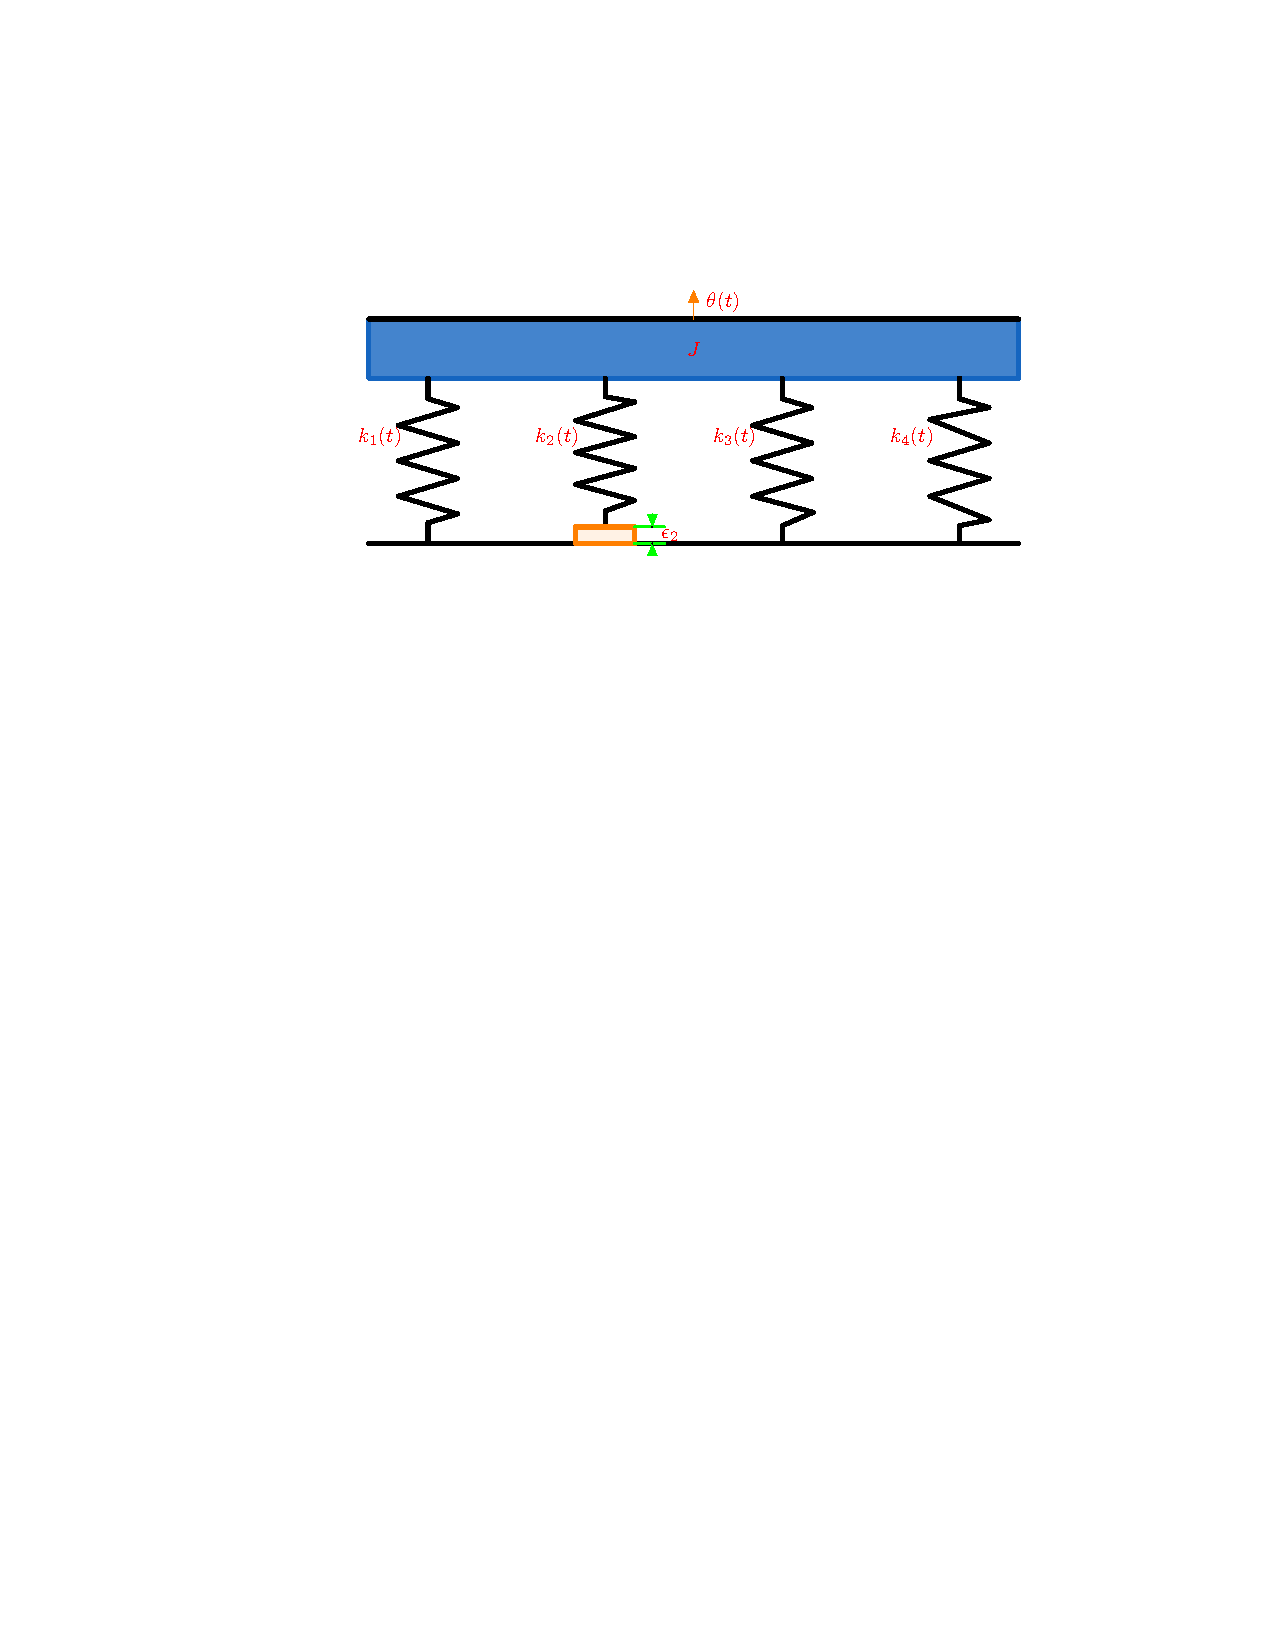
\includegraphics[scale=0.6,width=0.8\textwidth,height=1.6in]{spring_mass.pdf}
        \caption{Vibration system of unequal load sharing among four planets.}
        \label{fig:vibration_system_of_spring_mass}
    \end{figure*}
\end{enumerate}
\subsection{Planetary structure}
\par A typical layout of planetary gearboxes consists of three kinds of gears mounted so that the centers of planet gears revolves around the center of sun and ring gears, as shown in Fig. \ref{fig:planetary_gearbox_layout}. This paper merely discusses the common cases of speed reducers where the sun gear connects with the power input shaft and the carrier works as power output, while vibration sensors are usually mounted on the surface of the stationary ring gear in diagnostic applications. 
\begin{figure}[pos=htbp]
    \centering
    \begin{annotate}{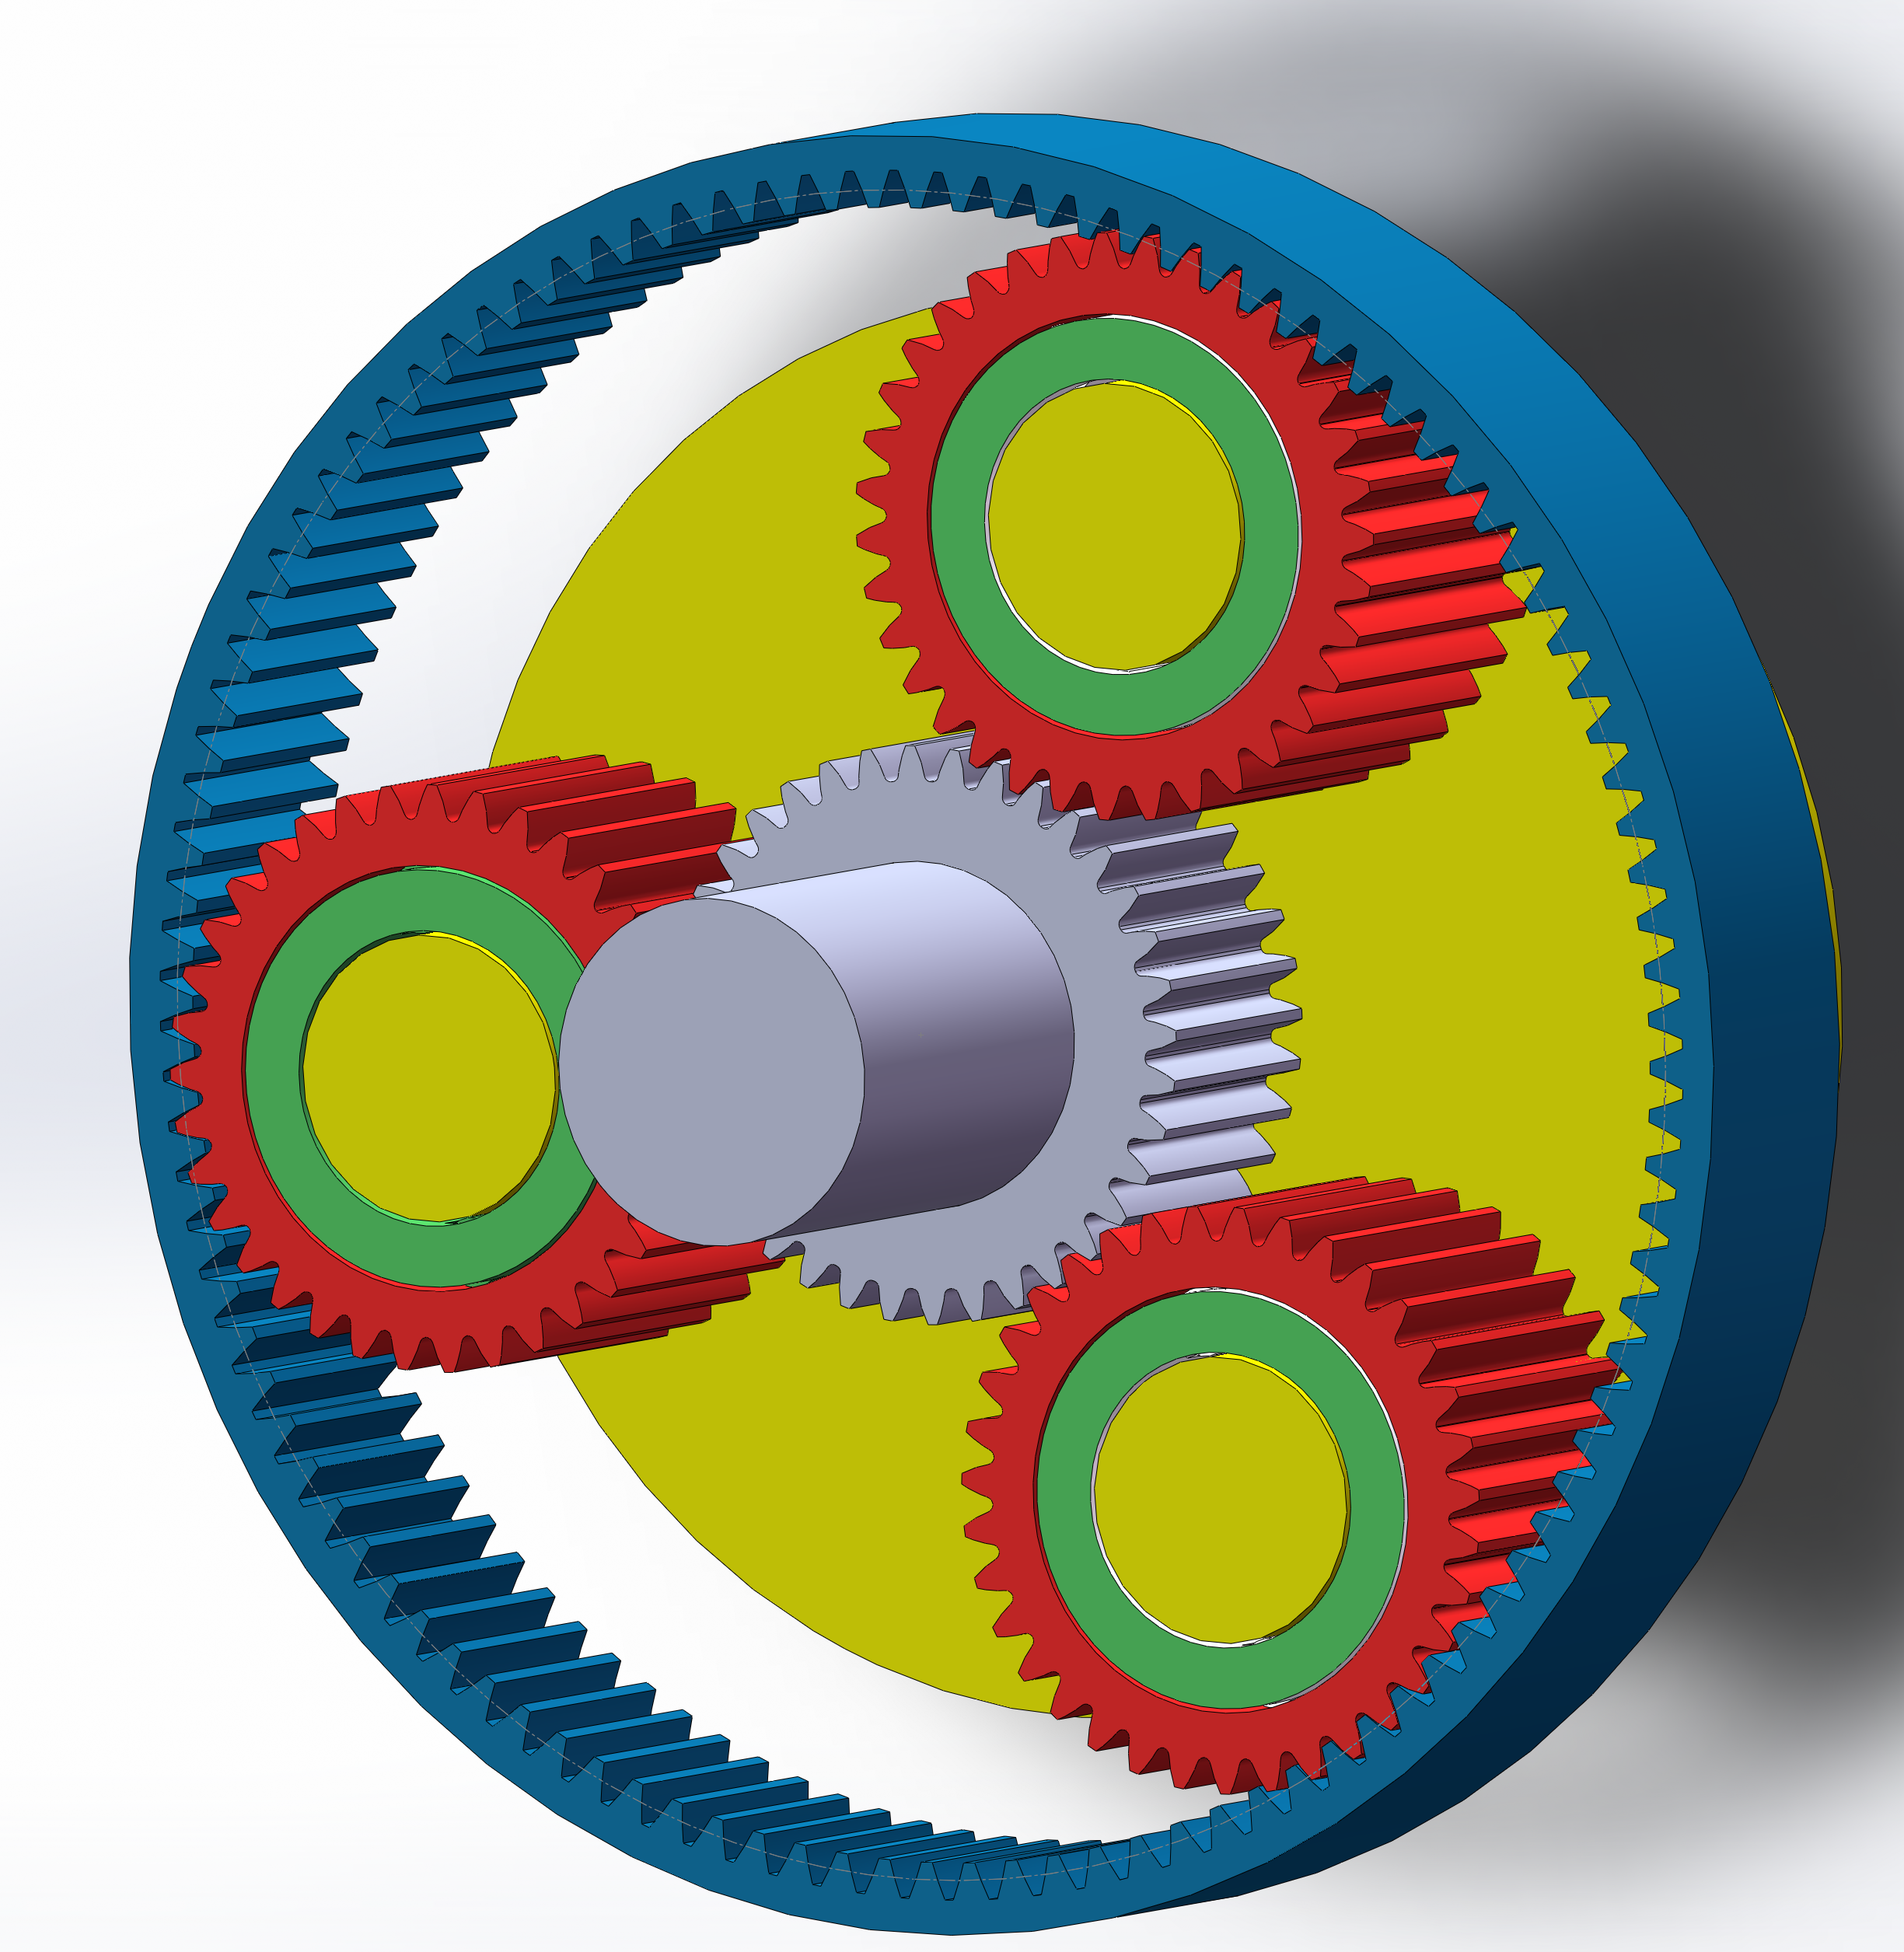
\includegraphics[width=0.3\textwidth]{Planetary_Gearbox.PNG}}{0.3}
        \callout{-8,-7}{Ring gear}{-5,-5.8}
        \callout{8,-7}{Planet gear}{4,-5.5}
        \callout{-8,7}{Sun gear}{-0.8,1.2}
        \callout{8,7}{Carrier}{4.5,1}
    \end{annotate}
    \caption{Configuration of planetary gearboxes.}
    \label{fig:planetary_gearbox_layout}
\end{figure}
\par The vibration in planetary gearboxes mainly origins from the meshing of gears \cite{Velex1996}. When the planet gears engage with the ring gear or sun gear, the number of the involved tooth varies with the relative rotation between gears and their contact stiffness changes consequently. The transmission load nominally remains constant and the gearbox is a parametrically excited multi-degree-freedom system \cite{Acar2019}. 
\subsection{Vibration of single planets}
\par To figure out the vibration mechanism of planetary gearboxes, we start with the meshing vibration of a pair of gears. For an individual planet, the vibration model can be written as
\begin{equation}
    J \cdot \ddot{\theta}(t) + k(t) \cdot \theta(t) = 0 \label{eq:1_DOF_vibration},
\end{equation}
where \(J\) is rotational inertia of the machine, \(\theta(t)\) is the shaft angular, \(\ddot{\theta}(t)\) is the rotational acceleration, \(k(t)\) is time-varying meshing stiffness and fluctuates in the form
\begin{equation}
    k(t)=k_0+2 q \cos(2 \pi f_{\rm m} t) \label{eq:meshing_stiffness},
\end{equation}
where \(k_0\) is the nominal meshing frequency, \(q\) denotes the the fluctuation intensity, and \(f_{\rm m}\) is the meshing frequency. Substitute Eq. (\ref{eq:meshing_stiffness}) into the Eq. (\ref{eq:1_DOF_vibration}), we have
\begin{equation}
    J \cdot \ddot{\theta}(t) + \left[k_0+2 q \cos(2 \pi f_{\rm m} t)\right] \cdot \theta(t) = 0. \label{eq:mathieu_function}
\end{equation}
\par Eq. (\ref{eq:mathieu_function}) is the Mathieu function. According to the Floquet theory \cite{Arscott2014}, its general solution the product of an exponential part and a harmonic part. Taking damper into account, we only consider stable operation conditions so that harmonic solution is concentrated. The response of the model in Eq. (\ref{eq:mathieu_function}) has the same harmonic component \(\cos(2 \pi f_{\rm m})\). The oscillation of gear meshing stiffness primarily contributes the vibration of planetary gearboxes.
\section{Factors considered in the signal model}
\begin{enumerate}
    \item Mechanism of time-varying gear meshing stiffness and risen impulses. (Including sun-planet and ring-planet)
    \item Transfer path effect led by the carrier rotation.
    \item Unequal load sharing risen by the planet angular position error.
    \item Differences in the impulsive intensity of planets with sun and ring gears arisen from the position errors of planet. (Amplitude modulation of angular position error)
    \item Phase shifts of transfer path effect of planet position error. (Frequency modulation of angular position error)
    \item Effects of asyncrhonous meshing between sun-planet and ring-planet.
    \item Effects of asyncrhonous meshing among sun-planets or ring-planets.
    \item Natural vibration influence on spectral structure.
\end{enumerate}

%% `Elsevier LaTeX' style
\bibliographystyle{elsarticle-num}
\bibliography{My_EndNote_Lib.bib}

\end{document}